\subsubsection{Begriffe}\label{containers_begriffe}

Um die Zusammenhänge in dieser Arbeit erläutern zu können, werden die folgenden Begriffe aus der Docker Terminologie benötigt:

\paragraph{Image}

Ein Image enthält die Applikation, sowie ihre Abhängigkeiten und Umgebungsvariablen zur Konfiguration des Containers.
Jeder Container wird auf Basis eines Images gestartet.
\footnote{What is a container image?, vgl.~\cite{DOCKER_CONTAINER_IMAGE}} \\

Images sind dabei in Schichten aufgebaut.
Ein Image hat also immer ein Basisimage.
Dieses wird im Dockerfile des Images mit dem Schlüsselwort \texttt{FROM} angegeben.
Jede Schicht eine Images ist eine Sammlung von Dateien, die es ermöglichen einen Container zu starten.
\footnote{A Beginner’s Guide to Understanding and Building Docker Images, vgl.~\cite{JFROG_CONTAINER_IMAGES}} \\

Es gibt zwei Wege ein Docker Image zu erstellen:

\begin{itemize}
    \item \textbf{Interaktiv:}
    Es wird ein Docker Container gestartet und manuell angepasst, anschließend lässt sich aus dem laufenden Container ein neues Image erstellen.

    \item \textbf{Dockerfile:}
    Das Image wird in einer Textdatei beschrieben, dazu stehen verschiedene Kommandos zur Verfügung.
    Diese erlauben es jede Art von Konfiguration vorzunehmen.
\end{itemize}

Ein Dockerfile ist dabei der \textit{reproduzierbare} Weg für die Erstellung eines Docker Images.
Mithilfe eines Dockerfiles können Images im Rahmen einer CI/CD Pipeline erstellt werden.

\paragraph{Registry}

Eine Container Registry wird verwendet, um Images zu publizieren und somit für andere Benutzer zur Verfügung zu stellen.
\footnote{About Registry, vgl.~\cite{DOCKER_ABOUT_REGISTRY}} \\

Die offizielle Registry unter hub.docker.com ist die größte öffentliche Registry.
Falls es nicht anders angegeben wird, versucht der Docker Client Images aus dieser Registry herunterzuladen.

Die Versionierung von Images wird dabei über Tags vorgenommen.
Ein Kommando wie \texttt{docker pull mysql} würde dabei das Image herunterladen dessen Tag \texttt{latest} ist. \\

Zur Festlegung einer Version kann z.B. das Kommando \texttt{docker pull mysql:8.0.22} verwendet werden.
Beim Veröffentlichen von Images über das Kommando \texttt{docker push} wird das Tag mit angegeben.
Falls nichts angegeben wird, erhält das neue Image automatisch das Tag \texttt{latest}.
\footnote{Docker Registry, vgl.~\cite{DOCKER_BASICS_REGISTRY}} \\

Um eigene Images zu veröffentlichen, kann man die Registry unter \href{https://hub.docker.com/}{hub.docker.com} verwenden oder auch einen eigenen Registry Server betreiben.
Für den Betrieb einer eigenen Registry gibt es ein offizielles Docker Image, welches einen Registry Server startet.
\footnote{Deploy a registry server, vgl.~\cite{DOCKER_DEPLOY_REGISTRY}} \\

Darüber hinaus gibt es zahlreiche weitere Anbieter, die es einem erlauben eine private Docker Image Registry zu betreiben.

\paragraph{Container}

Ein Container ist ein Prozess auf einem Docker Host.
Dieser Container wird immer auf Basis eines Image gestartet und stellt somit eine Instanz eines Image dar.
\footnote{What is a Container?, vgl.~\cite{DOCKER_WEBSITE}}

Mehrere Container können auf einem Host System laufen.
Die Prozesse sind hierbei vom restlichen System isoliert.
\footnote{Singh et al., vgl.~\cite{Singh2017}~[S.804]}

Docker verwendet hierfür sogenannte \textit{control groups}.
Dadurch soll eine Beschränkung auf dem Host System für bestimmte Ressourcen erreicht werden.
\footnote{Docker overview, vgl.~\cite{DOCKER_OVERVIEW}} \\

In der Regel führt ein Container nur einen Prozess aus, der erste gestartete Prozess ist dabei die Anwendung.
Wird diese Anwendung beendet, so beendet sich der Container ebenfalls.
\footnote{What is a Container?, vgl.~\cite{DOCKER_WEBSITE}}

%Beim Starten eines Containers gibt es verschiedene Parameter mit denen der Container konfiguriert wird:
%\footnote{Docker run reference, vgl.~\cite{DOCKER_RUN_REFERENCE}}
%
%\begin{itemize}
%    \item \texttt{-d} Detached bestimmt, ob der Container im Hintergrund ausgeführt wird
%    \item \texttt{-p} erlaubt das Mapping von Container Ports auf Host System Ports
%    \item \texttt{-e} ermöglicht das Setzen von Umgebungsvariablen
%    \item \texttt{-v} zur Speicherung von persistenten Daten können Pfade vom Host in den Container durchgegeben werden.
%\end{itemize}
%
%Desweiteren gibt es noch zahlreiche weitere Parameter mit denen sich bspw. CPU, Arbeitsspeicherlimits oder Berechtigungen festlegen lassen. \\
%
%Um z.B. einen Datenbank Container zu starten, verwendet man folgenden Befehl:
%
%\lstset{language=bash}
%\begin{lstlisting}[frame=htrbl, caption={Starten eines Docker Containers}, label={lst:docker_container_start}]
%docker run \
%-v /my/own/datadir:/var/lib/mysql \
%-e MYSQL_ROOT_PASSWORD=password \
%-p 3306:3306 \
%-d mysql:latest
%\end{lstlisting}
%
%Durch das Mapping des Ordners wird dafür gesorgt, dass die Daten außerhalb des Containers auf dem Host-System gespeichert werden.
%Auf diese Art lassen sich Updates von Software vereinfachen.
%Die persistenten Daten werden dazu einfach wieder in den neuen Container gemappt.

\paragraph{Container Host / Docker Client}

Das Host-System ist das Betriebssystem auf dem die Container Engine läuft.
Üblicherweise handelt es sich dabei um eine virtuelle Maschine mit Linux basierendem Betriebssystem.
Im Falle von Docker läuft ein \textit{docker daemon}.

Dieser stellt eine REST API sowie einen Socket zur Verfügung und verwaltet die Images sowie Container.
\footnote{Docker overview, vgl.~\cite{DOCKER_OVERVIEW}}

Über diese Schnittstellen kann die Docker CLI Container auf die benötigten Dienste zugreifen.
\footnote{Docker overview, vgl.~\cite{DOCKER_OVERVIEW}}

\begin{figure}[htb]
    \centering
    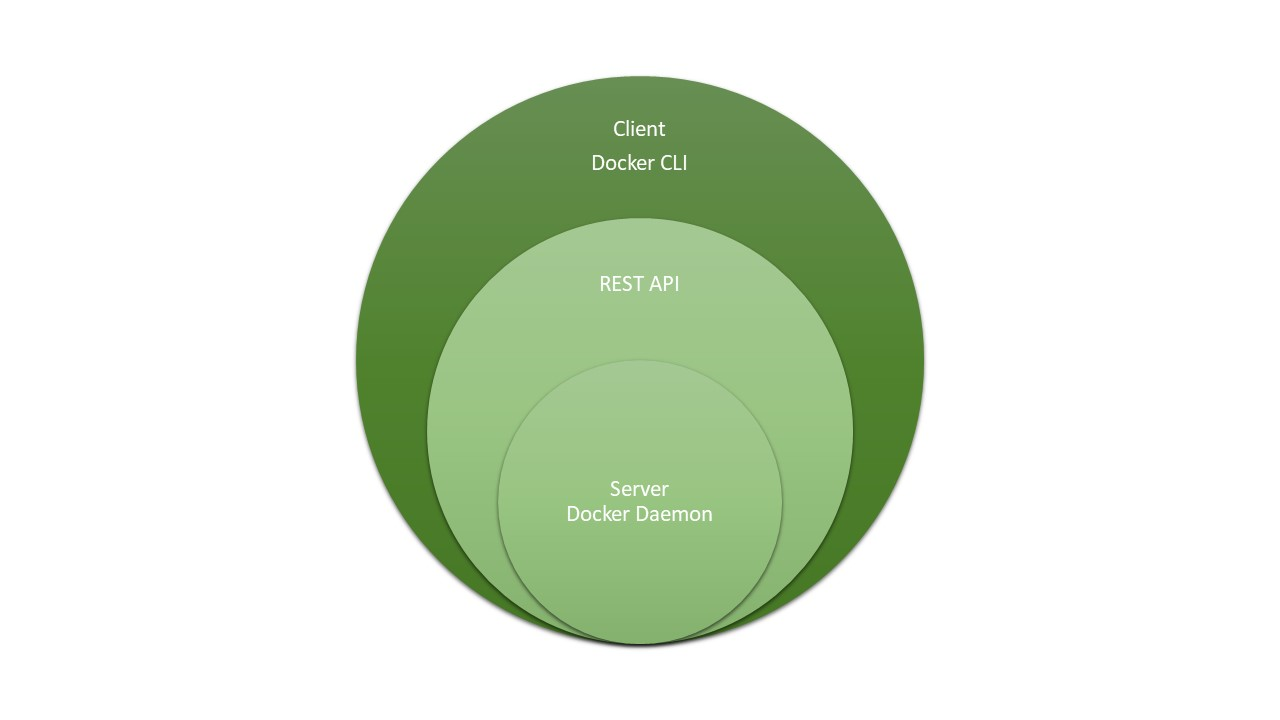
\includegraphics[width=0.7\textwidth]{images/docker_architecture.jpg}
    \caption[Docker Architektur]{Docker Architektur}
    \label{fig:Docker Architektur}
\end{figure}


Der Docker Client muss nicht zwingend auf dem Host-System laufen.
\footnote{Docker overview, vgl.~\cite{DOCKER_OVERVIEW}}

Es ist sogar möglich den Docker Socket in einen weiteren Container zu mounten und die Docker CLI innerhalb eines Containers zu verwenden, um Container auf dem Host-System zu verwalten.
\footnote{Singh et al., vgl.~\cite{Singh2017}~[S.806]}

% Über Client Zertifikatsauthentifizierung und HTTPS kann der Docker Client über das Internet verwendet werden, um einen Docker Host aus der Ferne zu verwalten.
% `(https://gist.github.com/kekru/974e40bb1cd4b947a53cca5ba4b0bbe5)`


